\documentclass[12pt,a4paper, ngerman, oneside]{scrartcl}
\usepackage[ngerman]{babel}
\usepackage[utf8]{inputenc}
%\usepackage[T1]{fontenc}
%\usepackage{lmodern}
\usepackage{ucs}
\usepackage{amsmath}
\usepackage{amsfonts}
\usepackage{amssymb}
\usepackage{graphics}
\usepackage{paralist}
\usepackage[linkcolor=black]{hyperref}
\usepackage{listings} \lstset{numbers=left, numberstyle=\tiny, numbersep=5pt} \lstset{language=Java}
%% Grafiken
\usepackage[pdftex]{graphicx}
\usepackage{epsfig} 
\hypersetup{% 
  colorlinks=true,
}

\newcommand\blfootnote[1]{%
  \begingroup
  \renewcommand\thefootnote{}\footnote{#1}%
  \addtocounter{footnote}{-1}%
  \endgroup
}

\hypersetup{
  pdfborder = {0 0 0},
  urlbordercolor = {0 0 0},
  colorlinks = true,
  linkcolor = black,
  citecolor = black,
  filecolor = black,
  urlcolor  = black
}
% Variablen
\newcommand{\Tiles}{\emph{8}}
\newcommand{\Rundenlimit}{\emph{20}}
\newcommand{\PointsPerTile}{\emph{7}}
\newcommand{\PointsPerPassenger}{\emph{7}}
\newcommand{\FieldsPerTile}{\emph{20}}
\newcommand{\Passagiere}{\emph{5}}


\sloppy
\hyphenpenalty=100000

\date{Software-Challenge Germany 2017\\Stand \today}


%\author{Niklas Paulsen, npau@informatik.uni-kiel.de }
\title{Spielanleitung Mississippi Queen}


\begin{document}
\maketitle
%\begin{figure}[!htbp]
%  \centering
%  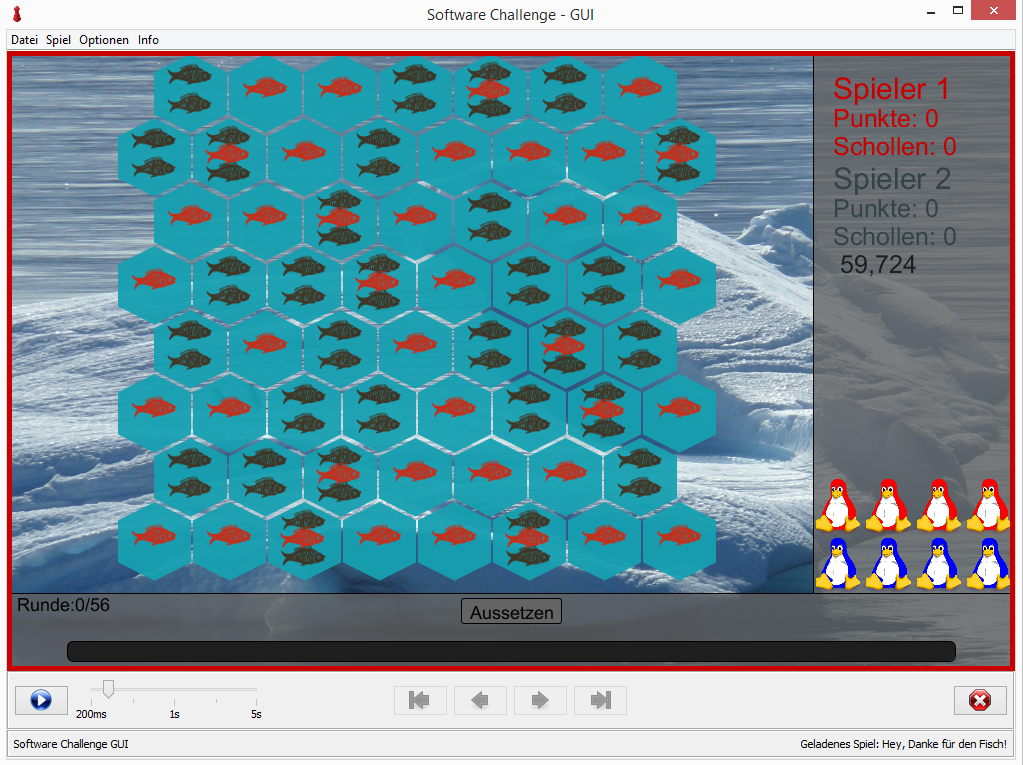
\includegraphics[width=\linewidth]{bilder/gui.png}
%\end{figure}
\vspace*{\fill}

%\blfootnote{Die Nutzung des Spielkonzeptes "`Twixt"' (Name, Spielregeln und Grafik)
%  erfolgt mit freundlicher Genehmigung des Kosmos Verlags.}

\newpage
\tableofcontents
\thispagestyle{empty}
\newpage
\setcounter{page}{1}
\section{Einleitung}
In dieser Anleitung werden die Elemente und Regeln des Spiels Mississippi Queen der
Software-Challenge 2017 erläutert.
Bei Mississippi Queen versuchen zwei Spieler, durch abwechselndes setzen von Raddampfern 
schnellstmöglich einen Fluss bis zum Ziel entlangzufahren und dabei zwei Passagiere mitzunehmen.
Der Spieler, der zuerst im Ziel gewinnt das Spiel.
\section{Das Spielbrett}
Ein Ausschnitt des Spielbretts ist im Titelbild zu sehen. Es besteht aus \emph{\Tiles} Spielsegmenten. Mit jeweils \emph{\FieldsPerTile} Feldern. Am Anfang ist das Startsegment und ein darauffolgendes Segment aufgedeckt. Sobald ein Spieler das letzte Segment betritt, wird ein neues dahinter zufällig links, rechts oder mittig angebaut. Dies geschieht solange, bis keine Segmente mehr übrig sind. Das letzte Segment ist das Zielsegment (TODO Graphik einfügen darin Zielfelder markieren). Segmente die schon von allen Spielern betreten wurden, werden vom Spielplan entfernt, auch wenn sich darauf noch Passagiere befinden.
Es gibt mehrere verschiedene Feldtypen:
\begin{itemize}
\item Das Wasserfeld (WATER) kann ganz normal befahren werden. Zu einem Wasserfeld zu ziehen kostet einen Geschwindigkeitspunkt.
\item Das Inselfeld (BLOCKED) kann nicht überquert werden.
\item Das Passagierfeld mt Anleger in Richtung i (PASSENGERi) enthält einen Passagier, der am entsprechenden Anleger abgeholt werden kann, wenn man das Feld mit Geschwindigkeit 1 erreicht.
\item Das Zielfeld (TARGET) ist ein Feld, dass erreicht werden kann, um das Spiel zu gewinnen.
\item Eine Sandbank (SANDBANK) bringt ein Schiff in der Bewegung zum halten, sollte man darauf fahren. Es kann nur rückwärts oder vorwärts dann aber unter Verwendung von einer Kohleeinheit verlassen werden.
\item Ein Baumstamm (LOG) ist ein Feld, das die doppelte Anzahl an Bewegungspunkten braucht, um es zu überqueren. Sind nicht genung Punkte vorhanden, kann es nicht überquert werden. TODO Bilder mit Feldern einfügen
\end{itemize}
Die Inselfelder sind dabei zufällig auf der Karte verteilt. Insgesamt gibt es \emph{\Passagiere} Passagierfelder. Sandbänke und Baumstämme werden ebenfalls zufällig eingefügt.
\section{Spielablauf}
Beide Spieler starten mit Geschwindigkeit 1 und 6 Kohleeinheiten und ziehen dann abwechselnd. Ein Zug sieht folgendermaßen aus:
\begin{itemize}
\item Falls vorhanden beginnt der Zug mit einer Änderung der Geschwindigkeit um +1 oder -1 (größere Beschleunigung ist durch Verwendung von jeweils einer Kohleeinheit pro Punkt möglich)
\item Darauf folgen beliebig viele Zug- oder Dreh-Aktionen oder eventuell Abdräng-Aktionen, solange genug Kohle vorhanden ist um sie durchzuführen. Dabei darf sich insgesamt nur so weit bewegt werden, wie Geschwindigkeitspunkte vorhanden sind. Eine Dreh-Aktion ist kostenlos, jede weitere Dreh-Aktion kostet eine Kohleeinheit.
\item Bei einer Abdräng-Aktion wird der gegnerische Spieler auf ein beliebiges angrenzendes Feld gestellt und der Gegner erhält für seinen nächsten Zug eine zusätzliche Dreh-Aktion.
\end{itemize} 
\section{Spielende}
Das Spiel endet, sobald ein Spieler mit 2 Passagieren ein Zielfeld erreicht hat oder sobald das Rundenlimit von \emph{\Rundenlimit} Runden erreicht ist. Wird das Rundenlimit erreicht gewinnt der Spieler mit den meisten Punkten. Die Punkte errechnen sich folgendermaßen:
\begin{itemize}
\item Jeder eingesammelte Passagier bringt 7 Punkte
\item Jedes Überwundene Segment bringt 7 Punkte. 
\item Anhang der Position innerhalb eines Segments werden 0 bis 6 Punkte vergeben. (Ein Segment ist aufgeteilt in 7 Reihen je weiter vorne man ist, desto mehr Punkte bekommt man TODO siehe Graphik).
\end{itemize}
Der Spieler mit den meisten Punkten gewinnt dann das Spiel.
\section{Graphische Benutzeroberfläche}
TODO

\end{document}
